\chapter{Project architecture}
\label{ch:architecture}
The described solution is composed of four directories with subprojects:
\begin{itemize}
\setlength\itemsep{0.2em}
\item data-gathering,
\item database-manager,
\item data-miner,
\item server,
\end{itemize}
three auto-generating directories with program-related data:
\begin{itemize}
\setlength\itemsep{0.2em}
\item logs,
\item flags,
\item data,
\end{itemize}
and a docker-compose.yml file. Each of the four directories has its own Dockerfile, and acts as a build context for that container image. Additionally, two containers are pulled from the Docker image repository, the MySQL server (\textit{mysql/mysql-server}) and Selenium standalone Firefox webdriver (\textit{selenium/standalone-firefox}).
Figure (\ref{arch:container_dependencies}) shows the dependencies between containers.

\begin{figure}[ht]
    \centering
    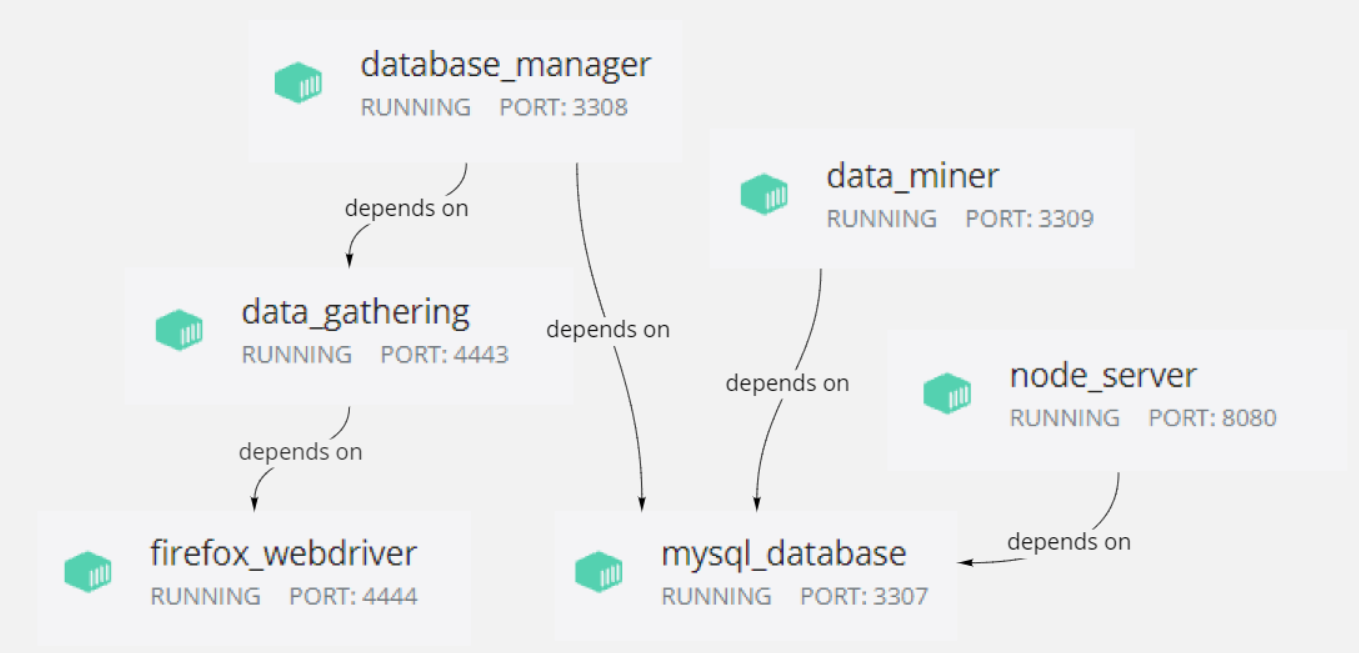
\includegraphics[width=\textwidth]{figures/container_dependencies.png}
    \caption{Boot order of containers (least dependant first)}
    \label{arch:container_dependencies}
\end{figure}

\section{Containers}
Issuing the \texttt{docker-compose up} command builds each local application image from a respective Dockerfile, and aranges them according to the configuration in docker-compose.yml file. All of the containers are booted to a shared network, with each container's name serving as an alias to be recognized immediately by other connected containers. Thus, every application exposes an internal port to the host via parameter: \par
\texttt{ports:} \par
\texttt{\qquad - "3308:3306"} \par
This notation indicates that port 3308 inside the container maps to port 3306 on the host. Additionally, to persist data between system composition and decomposition, docker volumes and data binds are used: \par
\texttt{volumes:} \par
\texttt{\qquad - ./data:/data} \par
\texttt{\qquad - ./logs:/logs} \par
\texttt{\qquad - ./flags:/flags} \par
\texttt{\qquad - pickle\_data:/.pickles} \par

Here, we declare that three directories relative to docker-compose.yml are supposed to be visible from the container's point of view as mounted in root directory. Any change to files inside the container will be immediately seen from the host level, providing the ability for several containers to work on a shared set of data. The pickles directory, on the other hand, is mapped to a \textit{named Docker volume}, that is virtual space managed by the containerization software. These volumes are persistent and very fast, but there is no way to peek at their contents. Only the running container can acccess the data there, therefore it acts perfectly as a space for files that should only be accessed by given container. \par
All of the containers also restart automatically on failure and share a set timezone. To stop the operation of the system, one can stop the app in Docker Desktop, or stop any of the containers, or delete them altogether. However, images created during the build will still exist, so to fully remove the app one can issue a command \texttt{docker-compose down --rmi local -v}, which stops and removes all containers, removes all local images, networks and volumes.

\subsection{Container: \textit{firefox\_webdriver}}
The \textit{firefox\_webdriver} container exposes port 4444 to send the traffic to the server through. It has no persistent memory and in general behaves like an abstract version of a Firefox browser running in the background, operated by any script that connects to it.

\subsection{Container: \textit{mysql\_database}}
Container \textit{mysql\_database} exposes hosts a database with persistent memory, storing the major part of the data warehouse and making it accessible to other containers.

\subsection{Container: \textit{data\_gathering}}
This subsystem automatically collects the web-scraped data in the \textit{data} directory

\subsection{Container: \textit{database\_manager}}
This takes this data and passes it to the database. It is important for the \textit{database\_manager} to be slightly delayed with respect to \textit{data\_gathering}

\subsection{Container: \textit{data\_miner}}
These containers are dependent only on the database, however here boot order or system state are not as important; these asynchonous containers perform their job properly when the data is ready and don't cause critial failure when it's not, which is enough for the system to run reliably.

\subsection{Container: \textit{node\_server}}
These containers are dependent only on the database, however here boot order or system state are not as important; these asynchonous containers perform their job properly when the data is ready and don't cause critial failure when it's not, which is enough for the system to run reliably.

\subsection{Container orchestration}
\label{container_orchestration}
The containers are all started when the \texttt{docker-compose up} command is issued in a root directory of the project. This causes the containers from external images to be loaded first, based on the dependency tree. From there, more control over the mutual cooridation is available via healthchecks or timing. Out of simplicity, the second approach has been selected for this thesis; i.e. the gathering project is initialized with an immediate 10 seconds delay, so that the webdriver is surely ready before a connection attempt takes place. Similarly, the database managing part is started after 20 seconds, so that the previous container can assess whether there is some new data and any action is needed, or that data can be verified, and marked as ready to be updated to the database. The data mining part is delayed 30 seconds, in case the database is in pre-update state, and other services will start to act on it. However, the most important element of orchestration is shared access to the flags directory, which stores two files with directory checksums, calculated from the ready and complete data after a gathering run. This checksum becomes the new standard and an indicator that the database contents may be outdated.


\section{Services}
The three programs written in Python share similar functions. These are grouped into \textbf{services} by their main utility and by needed external libraries. Each directory contains a \textit{services} module with the following:
\begin{itemize}
\setlength\itemsep{0.3em}
\item \textit{logs\_service} --- responsible for creating a container-specific logs directory with a daily log file and optionally run log file, general logging to file and console. Libraries needed: \textbf{os}, \textbf{time}.
\item \textit{flags\_service} --- this service creates the flags directory, sets up checksum files and provides an interface for everything related to detecting differences in directories or checking the current stage of the data. Libraries needed: \textbf{os}, \textbf{checksumdir}.
\item \textit{data\_service} --- handles everything related to CSV files, translating the scraped data into attributes, loading and saving dataframes, pickling and unpickling the data, all data manipulation pre-mining and ensuring the completeness and correctness of the data. Libraries needed: \textbf{os}, \textbf{sys}, \textbf{shutil}, \textbf{time}, \textbf{pandas}.
\item \textit{web\_service} --- interface for connecting to the webdriver and navigating the pages, finding appropriate elements on the website, implicit and explicit waiting for response, page validation and so on. Libraries needed: \textbf{time}, \textbf{bs4}, \textbf{selenium}.
\item \textit{database\_service} --- manages connection to the database, setting up the tables, updating the schema with new data, as well as creating helper views and additional tables in the data mining part. Libraries needed: \textbf{mysql.connector}.
\end{itemize}

\section{Data pipeline}
High level overview of the data pipeline (schema).
Where does the data come from? How do I get it?
Where do I validate it? What happens in the directories?
What happens in Docker volumes? What happens in the database?
What is the end result of the pipeline?
What is the speed of consecutive steps?

\begin{figure}[ht]
\centering
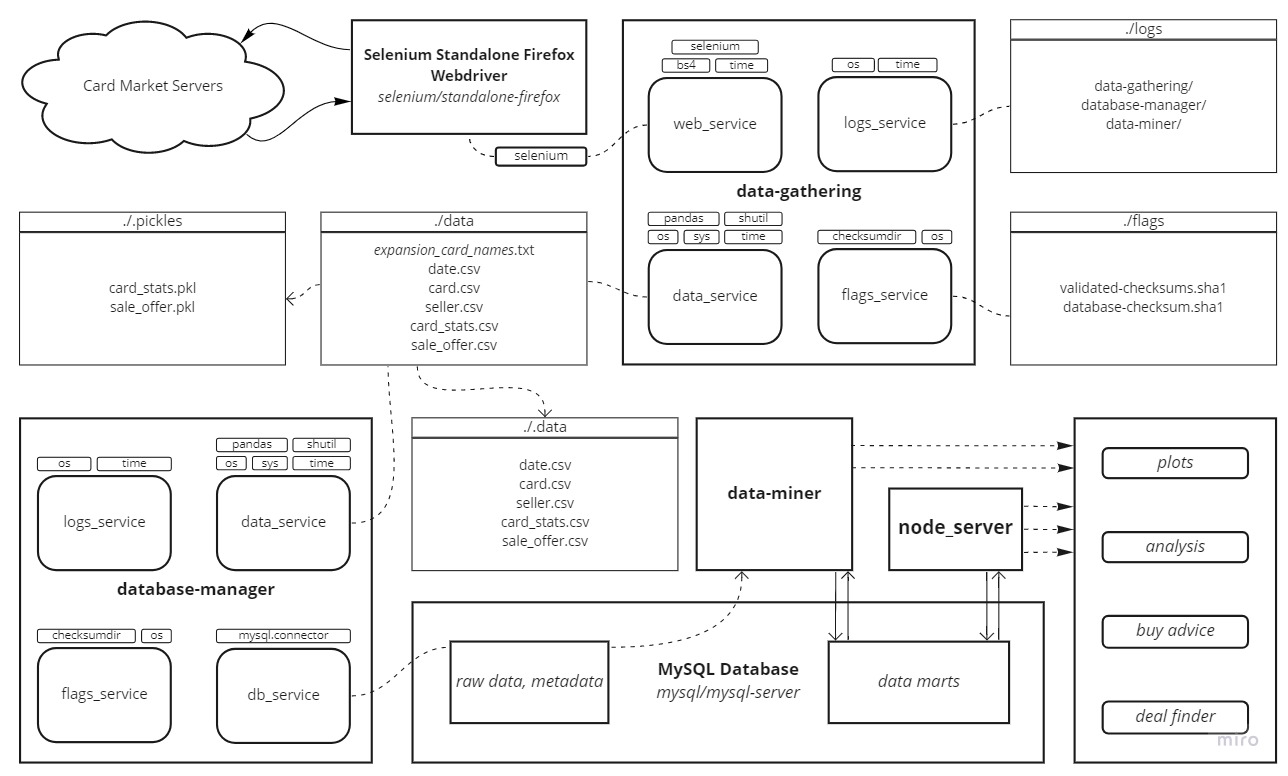
\includegraphics[width=\textwidth]{figures/warehousing.jpg}
\caption{Data pipeline from the server (left-top) to results (right-bottom).}
\end{figure}


\section{Compatilibity}
Is my project compatible with main operating systems?
How does the installation differ on various systems?

